\documentclass[1p]{elsarticle_modified}
%\bibliographystyle{elsarticle-num}

%\usepackage[colorlinks]{hyperref}
%\usepackage{abbrmath_seonhwa} %\Abb, \Ascr, \Acal ,\Abf, \Afrak
\usepackage{amsfonts}
\usepackage{amssymb}
\usepackage{amsmath}
\usepackage{amsthm}
\usepackage{scalefnt}
\usepackage{amsbsy}
\usepackage{kotex}
\usepackage{caption}
\usepackage{subfig}
\usepackage{color}
\usepackage{graphicx}
\usepackage{xcolor} %% white, black, red, green, blue, cyan, magenta, yellow
\usepackage{float}
\usepackage{setspace}
\usepackage{hyperref}

\usepackage{tikz}
\usetikzlibrary{arrows}

\usepackage{multirow}
\usepackage{array} % fixed length table
\usepackage{hhline}

%%%%%%%%%%%%%%%%%%%%%
\makeatletter
\renewcommand*\env@matrix[1][\arraystretch]{%
	\edef\arraystretch{#1}%
	\hskip -\arraycolsep
	\let\@ifnextchar\new@ifnextchar
	\array{*\c@MaxMatrixCols c}}
\makeatother %https://tex.stackexchange.com/questions/14071/how-can-i-increase-the-line-spacing-in-a-matrix
%%%%%%%%%%%%%%%

\usepackage[normalem]{ulem}

\newcommand{\msout}[1]{\ifmmode\text{\sout{\ensuremath{#1}}}\else\sout{#1}\fi}
%SOURCE: \msout is \stkout macro in https://tex.stackexchange.com/questions/20609/strikeout-in-math-mode

\newcommand{\cancel}[1]{
	\ifmmode
	{\color{red}\msout{#1}}
	\else
	{\color{red}\sout{#1}}
	\fi
}

\newcommand{\add}[1]{
	{\color{blue}\uwave{#1}}
}

\newcommand{\replace}[2]{
	\ifmmode
	{\color{red}\msout{#1}}{\color{blue}\uwave{#2}}
	\else
	{\color{red}\sout{#1}}{\color{blue}\uwave{#2}}
	\fi
}

\newcommand{\Sol}{\mathcal{S}} %segment
\newcommand{\D}{D} %diagram
\newcommand{\A}{\mathcal{A}} %arc


%%%%%%%%%%%%%%%%%%%%%%%%%%%%%5 test

\def\sl{\operatorname{\textup{SL}}(2,\Cbb)}
\def\psl{\operatorname{\textup{PSL}}(2,\Cbb)}
\def\quan{\mkern 1mu \triangleright \mkern 1mu}

\theoremstyle{definition}
\newtheorem{thm}{Theorem}[section]
\newtheorem{prop}[thm]{Proposition}
\newtheorem{lem}[thm]{Lemma}
\newtheorem{ques}[thm]{Question}
\newtheorem{cor}[thm]{Corollary}
\newtheorem{defn}[thm]{Definition}
\newtheorem{exam}[thm]{Example}
\newtheorem{rmk}[thm]{Remark}
\newtheorem{alg}[thm]{Algorithm}

\newcommand{\I}{\sqrt{-1}}
\begin{document}

%\begin{frontmatter}
%
%\title{Boundary parabolic representations of knots up to 8 crossings}
%
%%% Group authors per affiliation:
%\author{Yunhi Cho} 
%\address{Department of Mathematics, University of Seoul, Seoul, Korea}
%\ead{yhcho@uos.ac.kr}
%
%
%\author{Seonhwa Kim} %\fnref{s_kim}}
%\address{Center for Geometry and Physics, Institute for Basic Science, Pohang, 37673, Korea}
%\ead{ryeona17@ibs.re.kr}
%
%\author{Hyuk Kim}
%\address{Department of Mathematical Sciences, Seoul National University, Seoul 08826, Korea}
%\ead{hyukkim@snu.ac.kr}
%
%\author{Seokbeom Yoon}
%\address{Department of Mathematical Sciences, Seoul National University, Seoul, 08826,  Korea}
%\ead{sbyoon15@snu.ac.kr}
%
%\begin{abstract}
%We find all boundary parabolic representation of knots up to 8 crossings.
%
%\end{abstract}
%\begin{keyword}
%    \MSC[2010] 57M25 
%\end{keyword}
%
%\end{frontmatter}

%\linenumbers
%\tableofcontents
%
\newcommand\colored[1]{\textcolor{white}{\rule[-0.35ex]{0.8em}{1.4ex}}\kern-0.8em\color{red} #1}%
%\newcommand\colored[1]{\textcolor{white}{ #1}\kern-2.17ex	\textcolor{white}{ #1}\kern-1.81ex	\textcolor{white}{ #1}\kern-2.15ex\color{red}#1	}

{\Large $\underline{12a_{0532}~(K12a_{0532})}$}

\setlength{\tabcolsep}{10pt}
\renewcommand{\arraystretch}{1.6}
\vspace{1cm}\begin{tabular}{m{100pt}>{\centering\arraybackslash}m{274pt}}
\multirow{5}{120pt}{
	\centering
	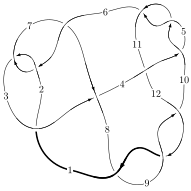
\includegraphics[width=112pt]{../../../GIT/diagram.site/Diagrams/png/1333_12a_0532.png}\\
\ \ \ A knot diagram\footnotemark}&
\allowdisplaybreaks
\textbf{Linearized knot diagam} \\
\cline{2-2}
 &
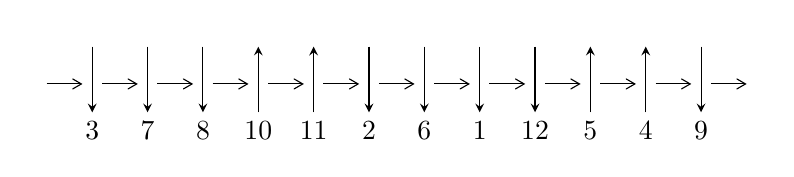
\begin{tikzpicture}[x=20pt, y=17pt]
	% nodes
	\node (C0) at (0, 0) {};
	\node (C1) at (1, 0) {};
	\node (C1U) at (1, +1) {};
	\node (C1D) at (1, -1) {3};

	\node (C2) at (2, 0) {};
	\node (C2U) at (2, +1) {};
	\node (C2D) at (2, -1) {7};

	\node (C3) at (3, 0) {};
	\node (C3U) at (3, +1) {};
	\node (C3D) at (3, -1) {8};

	\node (C4) at (4, 0) {};
	\node (C4U) at (4, +1) {};
	\node (C4D) at (4, -1) {10};

	\node (C5) at (5, 0) {};
	\node (C5U) at (5, +1) {};
	\node (C5D) at (5, -1) {11};

	\node (C6) at (6, 0) {};
	\node (C6U) at (6, +1) {};
	\node (C6D) at (6, -1) {2};

	\node (C7) at (7, 0) {};
	\node (C7U) at (7, +1) {};
	\node (C7D) at (7, -1) {6};

	\node (C8) at (8, 0) {};
	\node (C8U) at (8, +1) {};
	\node (C8D) at (8, -1) {1};

	\node (C9) at (9, 0) {};
	\node (C9U) at (9, +1) {};
	\node (C9D) at (9, -1) {12};

	\node (C10) at (10, 0) {};
	\node (C10U) at (10, +1) {};
	\node (C10D) at (10, -1) {5};

	\node (C11) at (11, 0) {};
	\node (C11U) at (11, +1) {};
	\node (C11D) at (11, -1) {4};

	\node (C12) at (12, 0) {};
	\node (C12U) at (12, +1) {};
	\node (C12D) at (12, -1) {9};
	\node (C13) at (13, 0) {};

	% arrows
	\draw[->,>={angle 60}]
	(C0) edge (C1) (C1) edge (C2) (C2) edge (C3) (C3) edge (C4) (C4) edge (C5) (C5) edge (C6) (C6) edge (C7) (C7) edge (C8) (C8) edge (C9) (C9) edge (C10) (C10) edge (C11) (C11) edge (C12) (C12) edge (C13) ;	\draw[->,>=stealth]
	(C1U) edge (C1D) (C2U) edge (C2D) (C3U) edge (C3D) (C4D) edge (C4U) (C5D) edge (C5U) (C6U) edge (C6D) (C7U) edge (C7D) (C8U) edge (C8D) (C9U) edge (C9D) (C10D) edge (C10U) (C11D) edge (C11U) (C12U) edge (C12D) ;
	\end{tikzpicture} \\
\hhline{~~} \\& 
\textbf{Solving Sequence} \\ \cline{2-2} 
 &
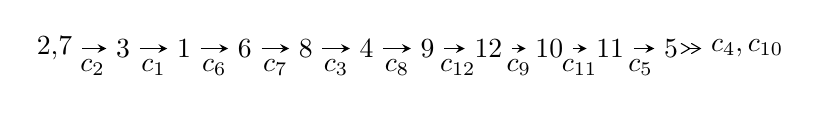
\begin{tikzpicture}[x=22pt, y=7pt]
	% node
	\node (A0) at (-1/8, 0) {2,7};
	\node (A1) at (1, 0) {3};
	\node (A2) at (2, 0) {1};
	\node (A3) at (3, 0) {6};
	\node (A4) at (4, 0) {8};
	\node (A5) at (5, 0) {4};
	\node (A6) at (6, 0) {9};
	\node (A7) at (7, 0) {12};
	\node (A8) at (8, 0) {10};
	\node (A9) at (9, 0) {11};
	\node (A10) at (10, 0) {5};
	\node (C1) at (1/2, -1) {$c_{2}$};
	\node (C2) at (3/2, -1) {$c_{1}$};
	\node (C3) at (5/2, -1) {$c_{6}$};
	\node (C4) at (7/2, -1) {$c_{7}$};
	\node (C5) at (9/2, -1) {$c_{3}$};
	\node (C6) at (11/2, -1) {$c_{8}$};
	\node (C7) at (13/2, -1) {$c_{12}$};
	\node (C8) at (15/2, -1) {$c_{9}$};
	\node (C9) at (17/2, -1) {$c_{11}$};
	\node (C10) at (19/2, -1) {$c_{5}$};
	\node (A11) at (45/4, 0) {$c_{4},c_{10}$};

	% edge
	\draw[->,>=stealth]	
	(A0) edge (A1) (A1) edge (A2) (A2) edge (A3) (A3) edge (A4) (A4) edge (A5) (A5) edge (A6) (A6) edge (A7) (A7) edge (A8) (A8) edge (A9) (A9) edge (A10) ;
	\draw[->>,>={angle 60}]	
	(A10) edge (A11);
\end{tikzpicture} \\ 

\end{tabular} \\

\footnotetext{
The image of knot diagram is generated by the software ``\textbf{Draw programme}" developed by Andrew Bartholomew(\url{http://www.layer8.co.uk/maths/draw/index.htm\#Running-draw}), where we modified some parts for our purpose(\url{https://github.com/CATsTAILs/LinksPainter}).
}\phantom \\ \newline 
\centering \textbf{Ideals for irreducible components\footnotemark of $X_{\text{par}}$} 
 
\begin{align*}
I^u_{1}&=\langle 
u^{62}+u^{61}+\cdots+u+1\rangle \\
\\
\end{align*}
\raggedright * 1 irreducible components of $\dim_{\mathbb{C}}=0$, with total 62 representations.\\
\footnotetext{All coefficients of polynomials are rational numbers. But the coefficients are sometimes approximated in decimal forms when there is not enough margin.}
\newpage
\renewcommand{\arraystretch}{1}
\centering \section*{I. $I^u_{1}= \langle u^{62}+u^{61}+\cdots+u+1 \rangle$}
\flushleft \textbf{(i) Arc colorings}\\
\begin{tabular}{m{7pt} m{180pt} m{7pt} m{180pt} }
\flushright $a_{2}=$&$\begin{pmatrix}1\\0\end{pmatrix}$ \\
\flushright $a_{7}=$&$\begin{pmatrix}0\\u\end{pmatrix}$ \\
\flushright $a_{3}=$&$\begin{pmatrix}1\\u^2\end{pmatrix}$ \\
\flushright $a_{1}=$&$\begin{pmatrix}- u^2+1\\- u^4\end{pmatrix}$ \\
\flushright $a_{6}=$&$\begin{pmatrix}u\\u\end{pmatrix}$ \\
\flushright $a_{8}=$&$\begin{pmatrix}- u^3\\- u^3+u\end{pmatrix}$ \\
\flushright $a_{4}=$&$\begin{pmatrix}- u^8+u^6- u^4+1\\- u^8+2 u^6-2 u^4+2 u^2\end{pmatrix}$ \\
\flushright $a_{9}=$&$\begin{pmatrix}- u^9+2 u^7-3 u^5+2 u^3- u\\- u^{11}+u^9-2 u^7+u^5- u^3+u\end{pmatrix}$ \\
\flushright $a_{12}=$&$\begin{pmatrix}- u^{16}+3 u^{14}-7 u^{12}+10 u^{10}-11 u^8+8 u^6-4 u^4+1\\- u^{18}+2 u^{16}-5 u^{14}+6 u^{12}-7 u^{10}+6 u^8-4 u^6+2 u^4- u^2\end{pmatrix}$ \\
\flushright $a_{10}=$&$\begin{pmatrix}- u^{23}+4 u^{21}+\cdots+4 u^3-2 u\\- u^{25}+3 u^{23}+\cdots-3 u^5+u\end{pmatrix}$ \\
\flushright $a_{11}=$&$\begin{pmatrix}u^{34}-5 u^{32}+\cdots+3 u^2+1\\u^{34}-6 u^{32}+\cdots+8 u^4- u^2\end{pmatrix}$ \\
\flushright $a_{5}=$&$\begin{pmatrix}u^{56}-9 u^{54}+\cdots+2 u^2+1\\u^{58}-8 u^{56}+\cdots-6 u^4+u^2\end{pmatrix}$\\&\end{tabular}
\flushleft \textbf{(ii) Obstruction class $= -1$}\\~\\
\flushleft \textbf{(iii) Cusp Shapes $= 4 u^{60}-36 u^{58}+\cdots+4 u+2$}\\~\\
\newpage\renewcommand{\arraystretch}{1}
\flushleft \textbf{(iv) u-Polynomials at the component}\newline \\
\begin{tabular}{m{50pt}|m{274pt}}
Crossings & \hspace{64pt}u-Polynomials at each crossing \\
\hline $$\begin{aligned}c_{1},c_{7}\end{aligned}$$&$\begin{aligned}
&u^{62}+19 u^{61}+\cdots-3 u+1
\end{aligned}$\\
\hline $$\begin{aligned}c_{2},c_{6}\end{aligned}$$&$\begin{aligned}
&u^{62}- u^{61}+\cdots- u+1
\end{aligned}$\\
\hline $$\begin{aligned}c_{3}\end{aligned}$$&$\begin{aligned}
&u^{62}+u^{61}+\cdots-1604 u+676
\end{aligned}$\\
\hline $$\begin{aligned}c_{4},c_{5},c_{10}\end{aligned}$$&$\begin{aligned}
&u^{62}+u^{61}+\cdots+u+1
\end{aligned}$\\
\hline $$\begin{aligned}c_{8},c_{9},c_{12}\end{aligned}$$&$\begin{aligned}
&u^{62}-7 u^{61}+\cdots-255 u+23
\end{aligned}$\\
\hline $$\begin{aligned}c_{11}\end{aligned}$$&$\begin{aligned}
&u^{62}-3 u^{61}+\cdots+943 u-949
\end{aligned}$\\
\hline
\end{tabular}\\~\\
\newpage\renewcommand{\arraystretch}{1}
\flushleft \textbf{(v) Riley Polynomials at the component}\newline \\
\begin{tabular}{m{50pt}|m{274pt}}
Crossings & \hspace{64pt}Riley Polynomials at each crossing \\
\hline $$\begin{aligned}c_{1},c_{7}\end{aligned}$$&$\begin{aligned}
&y^{62}+49 y^{61}+\cdots+7 y+1
\end{aligned}$\\
\hline $$\begin{aligned}c_{2},c_{6}\end{aligned}$$&$\begin{aligned}
&y^{62}-19 y^{61}+\cdots+3 y+1
\end{aligned}$\\
\hline $$\begin{aligned}c_{3}\end{aligned}$$&$\begin{aligned}
&y^{62}+25 y^{61}+\cdots+6973656 y+456976
\end{aligned}$\\
\hline $$\begin{aligned}c_{4},c_{5},c_{10}\end{aligned}$$&$\begin{aligned}
&y^{62}-59 y^{61}+\cdots+3 y+1
\end{aligned}$\\
\hline $$\begin{aligned}c_{8},c_{9},c_{12}\end{aligned}$$&$\begin{aligned}
&y^{62}+69 y^{61}+\cdots+4527 y+529
\end{aligned}$\\
\hline $$\begin{aligned}c_{11}\end{aligned}$$&$\begin{aligned}
&y^{62}-31 y^{61}+\cdots-27237285 y+900601
\end{aligned}$\\
\hline
\end{tabular}\\~\\
\newpage\flushleft \textbf{(vi) Complex Volumes and Cusp Shapes}
$$\begin{array}{c|c|c}  
\text{Solutions to }I^u_{1}& \I (\text{vol} + \sqrt{-1}CS) & \text{Cusp shape}\\
 \hline 
\begin{aligned}
u &= \phantom{-}0.989985 + 0.122617 I\end{aligned}
 & \phantom{-}1.32863 - 4.99314 I & -5.10286 + 6.83275 I \\ \hline\begin{aligned}
u &= \phantom{-}0.989985 - 0.122617 I\end{aligned}
 & \phantom{-}1.32863 + 4.99314 I & -5.10286 - 6.83275 I \\ \hline\begin{aligned}
u &= -0.809064 + 0.581444 I\end{aligned}
 & \phantom{-}3.36810 - 0.06751 I & -1.94023 + 0.35609 I \\ \hline\begin{aligned}
u &= -0.809064 - 0.581444 I\end{aligned}
 & \phantom{-}3.36810 + 0.06751 I & -1.94023 - 0.35609 I \\ \hline\begin{aligned}
u &= \phantom{-}0.975055\phantom{ +0.000000I}\end{aligned}
 & -0.841645\phantom{ +0.000000I} & -8.82830\phantom{ +0.000000I} \\ \hline\begin{aligned}
u &= -0.962183 + 0.082730 I\end{aligned}
 & -3.35982 + 2.23077 I & -11.92321 - 6.16182 I \\ \hline\begin{aligned}
u &= -0.962183 - 0.082730 I\end{aligned}
 & -3.35982 - 2.23077 I & -11.92321 + 6.16182 I \\ \hline\begin{aligned}
u &= \phantom{-}0.734854 + 0.732067 I\end{aligned}
 & \phantom{-}2.04758 + 1.64642 I & -2.09598 - 4.37427 I \\ \hline\begin{aligned}
u &= \phantom{-}0.734854 - 0.732067 I\end{aligned}
 & \phantom{-}2.04758 - 1.64642 I & -2.09598 + 4.37427 I \\ \hline\begin{aligned}
u &= \phantom{-}1.007400 + 0.257971 I\end{aligned}
 & \phantom{-}3.02841 - 0.92384 I & -4.00000 + 0.56914 I \\ \hline\begin{aligned}
u &= \phantom{-}1.007400 - 0.257971 I\end{aligned}
 & \phantom{-}3.02841 + 0.92384 I & -4.00000 - 0.56914 I \\ \hline\begin{aligned}
u &= -0.714319 + 0.763961 I\end{aligned}
 & \phantom{-}7.22652 - 4.54026 I & \phantom{-}2.91659 + 4.06961 I \\ \hline\begin{aligned}
u &= -0.714319 - 0.763961 I\end{aligned}
 & \phantom{-}7.22652 + 4.54026 I & \phantom{-}2.91659 - 4.06961 I \\ \hline\begin{aligned}
u &= -1.021670 + 0.240610 I\end{aligned}
 & \phantom{-}2.88991 + 5.19815 I & -4.00000 - 6.77683 I \\ \hline\begin{aligned}
u &= -1.021670 - 0.240610 I\end{aligned}
 & \phantom{-}2.88991 - 5.19815 I & -4.00000 + 6.77683 I \\ \hline\begin{aligned}
u &= -1.015640 + 0.277475 I\end{aligned}
 & \phantom{-}9.38200 - 2.18146 I & \phantom{-0.000000 }      -6
0. 10   - 0.620626 I \\ \hline\begin{aligned}
u &= -1.015640 - 0.277475 I\end{aligned}
 & \phantom{-}9.38200 + 2.18146 I & \phantom{-0.000000 -}     -6
0. 10   + 0.620626 I \\ \hline\begin{aligned}
u &= \phantom{-}1.037690 + 0.240795 I\end{aligned}
 & \phantom{-}9.12317 - 8.49284 I & \phantom{-0.000000 -}0. + 6.46268 I \\ \hline\begin{aligned}
u &= \phantom{-}1.037690 - 0.240795 I\end{aligned}
 & \phantom{-}9.12317 + 8.49284 I & \phantom{-0.000000 } 0. - 6.46268 I \\ \hline\begin{aligned}
u &= -0.794505 + 0.726721 I\end{aligned}
 & \phantom{-}3.07799 + 1.41254 I & \phantom{-}2.04320 - 3.32582 I \\ \hline\begin{aligned}
u &= -0.794505 - 0.726721 I\end{aligned}
 & \phantom{-}3.07799 - 1.41254 I & \phantom{-}2.04320 + 3.32582 I \\ \hline\begin{aligned}
u &= \phantom{-}0.884379 + 0.631379 I\end{aligned}
 & -0.51363 - 2.45305 I & -8.70061 + 2.47945 I \\ \hline\begin{aligned}
u &= \phantom{-}0.884379 - 0.631379 I\end{aligned}
 & -0.51363 + 2.45305 I & -8.70061 - 2.47945 I \\ \hline\begin{aligned}
u &= \phantom{-}0.740332 + 0.843987 I\end{aligned}
 & \phantom{-}9.98619 + 4.42504 I & \phantom{-0.000000 } 0 \\ \hline\begin{aligned}
u &= \phantom{-}0.740332 - 0.843987 I\end{aligned}
 & \phantom{-}9.98619 - 4.42504 I & \phantom{-0.000000 } 0 \\ \hline\begin{aligned}
u &= \phantom{-}0.814940 + 0.773369 I\end{aligned}
 & \phantom{-}9.03131 - 2.95277 I & \phantom{-0.000000 } 0 \\ \hline\begin{aligned}
u &= \phantom{-}0.814940 - 0.773369 I\end{aligned}
 & \phantom{-}9.03131 + 2.95277 I & \phantom{-0.000000 } 0 \\ \hline\begin{aligned}
u &= -0.736127 + 0.850348 I\end{aligned}
 & \phantom{-}16.3081 - 7.8313 I & \phantom{-0.000000 } 0 \\ \hline\begin{aligned}
u &= -0.736127 - 0.850348 I\end{aligned}
 & \phantom{-}16.3081 + 7.8313 I & \phantom{-0.000000 } 0 \\ \hline\begin{aligned}
u &= -0.749447 + 0.842317 I\end{aligned}
 & \phantom{-}10.15460 + 0.03373 I & \phantom{-0.000000 } 0\\
 \hline 
 \end{array}$$\newpage$$\begin{array}{c|c|c}  
\text{Solutions to }I^u_{1}& \I (\text{vol} + \sqrt{-1}CS) & \text{Cusp shape}\\
 \hline 
\begin{aligned}
u &= -0.749447 - 0.842317 I\end{aligned}
 & \phantom{-}10.15460 - 0.03373 I & \phantom{-0.000000 } 0 \\ \hline\begin{aligned}
u &= \phantom{-}0.870586\phantom{ +0.000000I}\end{aligned}
 & -1.55742\phantom{ +0.000000I} & -4.71840\phantom{ +0.000000I} \\ \hline\begin{aligned}
u &= \phantom{-}0.756113 + 0.848275 I\end{aligned}
 & \phantom{-}16.6739 - 3.2136 I & \phantom{-0.000000 } 0 \\ \hline\begin{aligned}
u &= \phantom{-}0.756113 - 0.848275 I\end{aligned}
 & \phantom{-}16.6739 + 3.2136 I & \phantom{-0.000000 } 0 \\ \hline\begin{aligned}
u &= -0.935495 + 0.651467 I\end{aligned}
 & \phantom{-}2.87996 + 4.99342 I & \phantom{-0.000000 } 0 \\ \hline\begin{aligned}
u &= -0.935495 - 0.651467 I\end{aligned}
 & \phantom{-}2.87996 - 4.99342 I & \phantom{-0.000000 } 0 \\ \hline\begin{aligned}
u &= -0.930376 + 0.707827 I\end{aligned}
 & \phantom{-}2.66249 + 4.07137 I & \phantom{-0.000000 } 0 \\ \hline\begin{aligned}
u &= -0.930376 - 0.707827 I\end{aligned}
 & \phantom{-}2.66249 - 4.07137 I & \phantom{-0.000000 } 0 \\ \hline\begin{aligned}
u &= \phantom{-}0.926438 + 0.747239 I\end{aligned}
 & \phantom{-}8.69067 - 2.79047 I & \phantom{-0.000000 } 0 \\ \hline\begin{aligned}
u &= \phantom{-}0.926438 - 0.747239 I\end{aligned}
 & \phantom{-}8.69067 + 2.79047 I & \phantom{-0.000000 } 0 \\ \hline\begin{aligned}
u &= \phantom{-}0.965239 + 0.702224 I\end{aligned}
 & \phantom{-}1.35675 - 7.13213 I & \phantom{-0.000000 } 0 \\ \hline\begin{aligned}
u &= \phantom{-}0.965239 - 0.702224 I\end{aligned}
 & \phantom{-}1.35675 + 7.13213 I & \phantom{-0.000000 } 0 \\ \hline\begin{aligned}
u &= -0.982215 + 0.711411 I\end{aligned}
 & \phantom{-}6.42370 + 10.13930 I & \phantom{-0.000000 } 0 \\ \hline\begin{aligned}
u &= -0.982215 - 0.711411 I\end{aligned}
 & \phantom{-}6.42370 - 10.13930 I & \phantom{-0.000000 } 0 \\ \hline\begin{aligned}
u &= -0.995337 + 0.760558 I\end{aligned}
 & \phantom{-}9.39615 + 5.95109 I & \phantom{-0.000000 } 0 \\ \hline\begin{aligned}
u &= -0.995337 - 0.760558 I\end{aligned}
 & \phantom{-}9.39615 - 5.95109 I & \phantom{-0.000000 } 0 \\ \hline\begin{aligned}
u &= \phantom{-}1.001000 + 0.757438 I\end{aligned}
 & \phantom{-}9.18276 - 10.40390 I & \phantom{-0.000000 } 0 \\ \hline\begin{aligned}
u &= \phantom{-}1.001000 - 0.757438 I\end{aligned}
 & \phantom{-}9.18276 + 10.40390 I & \phantom{-0.000000 } 0 \\ \hline\begin{aligned}
u &= \phantom{-}0.994404 + 0.767003 I\end{aligned}
 & \phantom{-}15.9378 - 2.8100 I & \phantom{-0.000000 } 0 \\ \hline\begin{aligned}
u &= \phantom{-}0.994404 - 0.767003 I\end{aligned}
 & \phantom{-}15.9378 + 2.8100 I & \phantom{-0.000000 } 0 \\ \hline\begin{aligned}
u &= -1.005970 + 0.758828 I\end{aligned}
 & \phantom{-}15.4757 + 13.8328 I & \phantom{-0.000000 } 0 \\ \hline\begin{aligned}
u &= -1.005970 - 0.758828 I\end{aligned}
 & \phantom{-}15.4757 - 13.8328 I & \phantom{-0.000000 } 0 \\ \hline\begin{aligned}
u &= -0.620405 + 0.327589 I\end{aligned}
 & \phantom{-}3.29016 - 0.22305 I & -0.445284 - 1.174195 I \\ \hline\begin{aligned}
u &= -0.620405 - 0.327589 I\end{aligned}
 & \phantom{-}3.29016 + 0.22305 I & -0.445284 + 1.174195 I \\ \hline\begin{aligned}
u &= -0.024632 + 0.694041 I\end{aligned}
 & \phantom{-}12.57310 + 5.42065 I & \phantom{-}5.59415 - 3.08644 I \\ \hline\begin{aligned}
u &= -0.024632 - 0.694041 I\end{aligned}
 & \phantom{-}12.57310 - 5.42065 I & \phantom{-}5.59415 + 3.08644 I \\ \hline\begin{aligned}
u &= \phantom{-}0.012401 + 0.677140 I\end{aligned}
 & \phantom{-}6.22588 - 2.17623 I & \phantom{-}2.37812 + 3.15857 I \\ \hline\begin{aligned}
u &= \phantom{-}0.012401 - 0.677140 I\end{aligned}
 & \phantom{-}6.22588 + 2.17623 I & \phantom{-}2.37812 - 3.15857 I \\ \hline\begin{aligned}
u &= -0.163278 + 0.512817 I\end{aligned}
 & \phantom{-}4.83308 + 3.11441 I & \phantom{-}3.99348 - 4.97298 I \\ \hline\begin{aligned}
u &= -0.163278 - 0.512817 I\end{aligned}
 & \phantom{-}4.83308 - 3.11441 I & \phantom{-}3.99348 + 4.97298 I\\
 \hline 
 \end{array}$$\newpage$$\begin{array}{c|c|c}  
\text{Solutions to }I^u_{1}& \I (\text{vol} + \sqrt{-1}CS) & \text{Cusp shape}\\
 \hline 
\begin{aligned}
u &= \phantom{-}0.172662 + 0.354819 I\end{aligned}
 & -0.089492 - 0.934789 I & -1.87222 + 7.30268 I \\ \hline\begin{aligned}
u &= \phantom{-}0.172662 - 0.354819 I\end{aligned}
 & -0.089492 + 0.934789 I & -1.87222 - 7.30268 I\\
 \hline 
 \end{array}$$\newpage
\newpage\renewcommand{\arraystretch}{1}
\centering \section*{ II. u-Polynomials}
\begin{tabular}{m{50pt}|m{274pt}}
Crossings & \hspace{64pt}u-Polynomials at each crossing \\
\hline $$\begin{aligned}c_{1},c_{7}\end{aligned}$$&$\begin{aligned}
&u^{62}+19 u^{61}+\cdots-3 u+1
\end{aligned}$\\
\hline $$\begin{aligned}c_{2},c_{6}\end{aligned}$$&$\begin{aligned}
&u^{62}- u^{61}+\cdots- u+1
\end{aligned}$\\
\hline $$\begin{aligned}c_{3}\end{aligned}$$&$\begin{aligned}
&u^{62}+u^{61}+\cdots-1604 u+676
\end{aligned}$\\
\hline $$\begin{aligned}c_{4},c_{5},c_{10}\end{aligned}$$&$\begin{aligned}
&u^{62}+u^{61}+\cdots+u+1
\end{aligned}$\\
\hline $$\begin{aligned}c_{8},c_{9},c_{12}\end{aligned}$$&$\begin{aligned}
&u^{62}-7 u^{61}+\cdots-255 u+23
\end{aligned}$\\
\hline $$\begin{aligned}c_{11}\end{aligned}$$&$\begin{aligned}
&u^{62}-3 u^{61}+\cdots+943 u-949
\end{aligned}$\\
\hline
\end{tabular}\newpage\renewcommand{\arraystretch}{1}
\centering \section*{ III. Riley Polynomials}
\begin{tabular}{m{50pt}|m{274pt}}
Crossings & \hspace{64pt}Riley Polynomials at each crossing \\
\hline $$\begin{aligned}c_{1},c_{7}\end{aligned}$$&$\begin{aligned}
&y^{62}+49 y^{61}+\cdots+7 y+1
\end{aligned}$\\
\hline $$\begin{aligned}c_{2},c_{6}\end{aligned}$$&$\begin{aligned}
&y^{62}-19 y^{61}+\cdots+3 y+1
\end{aligned}$\\
\hline $$\begin{aligned}c_{3}\end{aligned}$$&$\begin{aligned}
&y^{62}+25 y^{61}+\cdots+6973656 y+456976
\end{aligned}$\\
\hline $$\begin{aligned}c_{4},c_{5},c_{10}\end{aligned}$$&$\begin{aligned}
&y^{62}-59 y^{61}+\cdots+3 y+1
\end{aligned}$\\
\hline $$\begin{aligned}c_{8},c_{9},c_{12}\end{aligned}$$&$\begin{aligned}
&y^{62}+69 y^{61}+\cdots+4527 y+529
\end{aligned}$\\
\hline $$\begin{aligned}c_{11}\end{aligned}$$&$\begin{aligned}
&y^{62}-31 y^{61}+\cdots-27237285 y+900601
\end{aligned}$\\
\hline
\end{tabular}
\vskip 2pc
\end{document}